\chapter{Comment organiser la base de tests et configurer l'application ?}
\label{configFile}
La configuration de l'application dépend grandement de l'architecture de la base de tests. Les images sont placées dans des répertoires correspondant idéalement à un type de code-barres. Le fichier de configuration est constitué de plusieurs lignes constituant chacune une instruction. Chaque instruction contient deux informations : le nom (ou une partie du nom) du répertoire appelé catégorie et le type de détection. On a donc le modèle suivant :
\\\verb|<catégorie> <type détection>|\\
Les deux informations ne doivent pas contenir d'espace et doivent être séparées par une espace. On peut choisir de référencer plusieurs répertoires par la même catégorie, il faudra dans ce cas que le nom des répertoires en question commencent par cette catégorie.

Pour chaque catégorie, on associe donc un type de détection qui indiquera à l'application quel algorithme de détection utiliser :
\begin{itemize}
 \item \og 1d \fg{} pour un code-barres 1D
 \item \og 2ddm \fg{} pour un code-barres DataMatrix
 \item \og 2dpdf \fg{} pour un code-barres PDF417
 \item \og qr \fg{} pour un QRcode
 \item \og all \fg{} pour une détection de tous les codes-barres précédents
\end{itemize}

Il est conseillé de limiter le nombre d'instructions en regroupant le plus possible les images. Vous obtiendrez ainsi une base de tests simple et claire. N'oubliez pas de créer pour chaque image un fichier du même nom (avec une extension .txt par exemple) qui servira de témoin. Même si l'image ne contient pas de code-barres (test de faux positifs) ou si la valeur de ce(s) codes-barres est inconnue, il faut au moins créer le fichier témoin. Il suffit ensuite de remplir ce fichier témoin à raison d'une valeur de code-barres par ligne.

Si ces conseils sont suivis, vous ne devriez pas rencontrer d'erreur lors du test de vos images.

\chapter{Comment une image est-elle traitée par l'application ?}

Afin de pouvoir analyser les informations contenues dans l'intégralité du jeu de test, il est nécessaire au préalable d'organiser ces informations. Plusieurs structures sont présentes pour assurer un agencement clair, et une traduction simple des données. Afin de décrire comment chacune entre en jeu, nous allons détailler un exemple de test.

\section{Détection}

\subsection{Principe}

Notre jeu de test est constitué d'un nombre \verb|n| d'images. Chaque image peut contenir un ou plusieurs codes-barres. Le processus de détection s'effectue dans la classe \verb|Model|. Lors de l'analyse d'une image, \verb|Model| crée un objet \verb|Barcode| par code-barres détecté, et le met dans un objet \verb|FileResult| qui correspond donc au résultat d'une détection pour un fichier.

\begin{figure}
\begin{center}
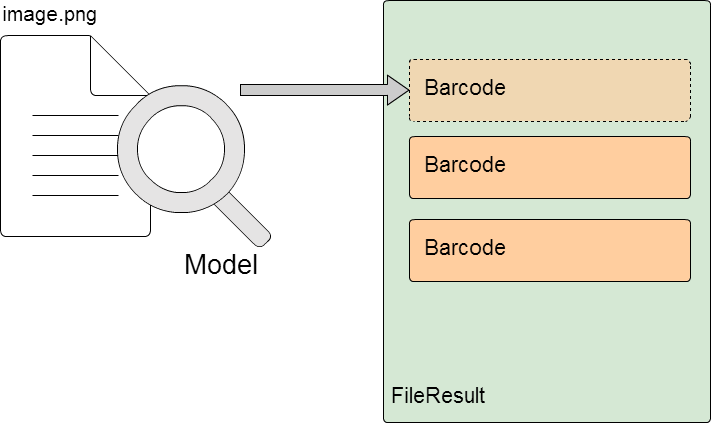
\includegraphics[scale=0.3]{images/projet1Detection.png}
\caption{Le processus d'analyse d'une image}
\end{center}
\end{figure}

Un objet \verb|Barcode| contient :
\begin{itemize}
\item La valeur du code-barres
\item Une valeur booléenne indiquant si le code-barres est correct au regard du fichier témoin de l'image
\item Le type du code-barres (1D, QRcode, etc.)
\end{itemize}

Un objet \verb|FileResult| contient bien sûr une liste de \verb|Barcode|, mais aussi :
\begin{itemize}
\item Le nom de l'image
\item Le nom du fichier témoin qui lui est associé
\item La catégorie, c'est à dire la valeur qui représente le répertoire de l'image dans le fichier de configuration
\item Le type de détection tel que spécifié dans le fichier de configuration
\item La liste des valeurs de controle contenues dans le fichier témoin
\item Un dictionnaire présentant l'état de la détection pour chaque type de codes-barres.
\end{itemize}

\subsection{Explication de code}

La classe \verb|Model| contient une méthode servant à la détection d'une image :\\\verb| DetectionError detectBarCode(string _nomFic, out FileResult file);|

Cette fonction prend en paramètre d'entrée le chemin de l'image. En paramètre de sortie, un objet de type \verb|FileResult| qui représente le résultat de la détection pour cette image. Cette fonction retourne une valeur de type \verb|DetectionError| qui est en fait une énumération à trois valeurs :
\begin{description}
\item[OK :] aucun problème détecté.
\item[CONTROL\_VALUE\_ERROR :] valeur de contrôle introuvable (lorsque le fichier témoin de l'image est introuvable ou mal nommé).
\item[DETECTION\_TYPE\_ERROR :] lorsque le répertoire de l'image n'est pas référencé dans le fichier de configuration.
\end{description}

Voici donc le contenu de cette fonction :
\newpage
\begin{lstlisting}
public DetectionError detectBarCode(string _nomFic, out FileResult file)
{
  file = new FileResult(_nomFic);
  file.CodeType = getCategory(file.Filename);
  file.DetectionType = getDetectionType(file.CodeType);

  // Checks if the detection type is correct
  if (file.DetectionType == String.Empty)
  {
    return DetectionError.DETECTION_TYPE_ERROR;
  }
  // Checks if the file test exists
  else if (!File.Exists(file.FilenameControl))
  {
    return DetectionError.CONTROL_VALUE_ERROR;
  }
  else
  {
    int image = this.gpi.CreateGdPictureImageFromFile(_nomFic);
    switch (file.DetectionType)
    {
      case "1d":
        detect1D(image, ref file)
        break;
      case "2ddm":
        detect2DDM(image, ref file);
        break;
      case "2dpdf":
        detect2DPDF(image, ref file);
        break;
      case "qr":
        detectQR(image, ref file);
        break;
      case "all":
        detect1D(image, ref file);
        detect2DDM(image, ref file);
        detect2DPDF(image, ref file);
        detectQR(image, ref file);
        break;
      default:
        break;
    }
    this.gpi.ReleaseGdPictureImage(image);
  }
  return DetectionError.OK;
}
\end{lstlisting}
\newpage

Et le commentaire des lignes importantes :
\begin{itemize}
\item[3-5 :] Création du \verb|FileResult| et initialisation de quelques attributs.
\item[19 :] Chargement du moteur de détection avec l'images à analyser. \verb|this.gpi| est un objet créé dans le constructeur de \verb|Model| et qui gère le dialogue entre l'application et le moteur de GdPicture. Il est détruit à la toute fin du test.
\item[20 :] Teste le type de détection définit dans le fichier de configuration. Il y a deux possibilités :
	\begin{itemize}
	\item Un type a été spécifié, on utilise donc la détection sur ce type.
	\item La valeur \emph{all} a été donnée, on fait donc une détection sur tous les types de codes-barres.
	\end{itemize}
\item[43 :] L'image est libérée en mémoire, on est prêt à passer à l'image suivante.
\end{itemize}

\paragraph{}

On remarque l'utilisation de la fonction \verb|detect*(image, ref file)|. En effet, suivant le type de détection, les fonctions de GdPicture à utiliser diffèrent. Voici un exemple avec la détection 1D :

\begin{lstlisting}
private FileResult detect1D(int image, ref FileResult file)
{
  this.gpi.Barcode1DReaderClear();
  Barcode result;
  file.DetectionStatus.Add("1d", this.gpi.Barcode1DReaderDoScan(image).ToString());
  int nbDetected = this.gpi.Barcode1DReaderGetBarcodeCount();
  for (int i = 0; i < nbDetected; i++)
  {
    result = new Barcode();
    result.barcode = gpi.Barcode1DReaderGetBarcodeValue(i + 1).Trim();
    result.detected = file.ControlBarcodes.Contains(result.barcode);
    result.detectionType = "1d";
    file.Barcodes.Add(result);
  }
  return file;
}
\end{lstlisting}

\begin{itemize}
\item[3 :] Nettoyage des éventuels précédentes détections
\item[5 :] Ajout de l'état de la détection renvoyé par la fonction de scan de GdPicture
\item[6 :] Récupération du nombre de codes-barres détectés
\item[7 :] Pour chaque code-barres, création d'un objet \verb|Barcode|, récupération de sa valeur et comparaison avec le fichier témoin. Ajout du code-barre au \verb|FileResult|.
\end{itemize}

On peut donc voir ici comment les codes-barres sont détectés et comment les résultats sont stockés dans des objets. Intéressons-nous maintenant à la création de rapports.

\section{Création de rapports}

La création de rapports s'effectue au sein de la classe Report. Son travail est de rassembler les résultats de tous les fichiers de la base de tests (contenus dans des \verb|FileResult|). Pour cela, elle crée un objet \verb|ReaderReport| qui représente un rapport, c'est à dire une analyse complète de la base de tests. En plus des informations de chaque fichier, elle contient des informations propres au rapport dans un objet \verb|ExtraReportInfo|. Elle parse ensuite le \verb|ReaderReport| dans un fichier JSON pour qu'il puisse être réutilisé.

\begin{figure}
\begin{center}
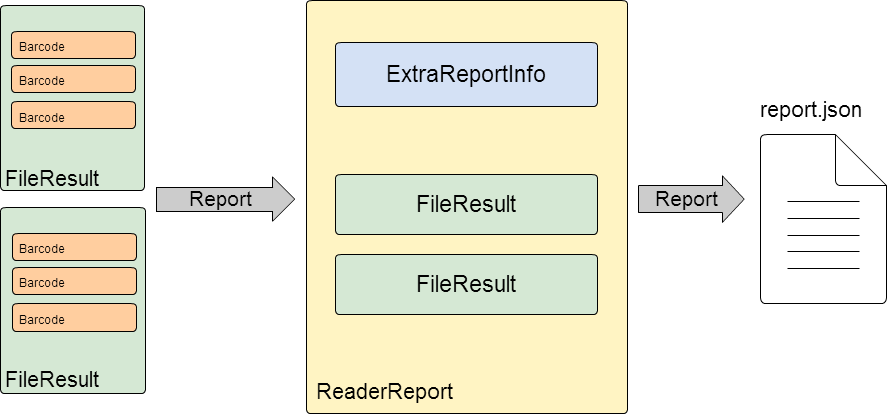
\includegraphics[scale=0.5]{images/projet1Rapport.png}
\caption{Le processus de création de rapport}
\end{center}
\end{figure}

Un objet \verb|ExtraReportInfo| contient plusieurs informations propres au rapport :
\begin{itemize}
\item La version courante de GdPicture
\item Une chaine représentant la date et l'heure de la détection
\item Le nombre de fichiers analysés
\item La liste des types de codes-barres connus
\item La liste des catégories (lié au fichier de configuration)
\end{itemize}